% !TEX TS-program = pdflatex
% !TEX encoding = UTF-8 Unicode

% This is a simple template for a LaTeX document using the "article" class.
% See "book", "report", "letter" for other types of document.

\documentclass[11pt]{article} % use larger type; default would be 10pt

\usepackage{amsmath}
\usepackage{amsfonts}
\usepackage[utf8]{inputenc} % set input encoding (not needed with XeLaTeX)

%%% Examples of Article customizations
% These packages are optional, depending whether you want the features they provide.
% See the LaTeX Companion or other references for full information.

%%% PAGE DIMENSIONS
\usepackage{geometry} % to change the page dimensions
\geometry{letterpaper} % or letterpaper (US) or a5paper or....
\geometry{margin=1in} % for example, change the margins to 2 inches all round
% \geometry{landscape} % set up the page for landscape
%   read geometry.pdf for detailed page layout information

\usepackage{graphicx} % support the \includegraphics command and options

% \usepackage[parfill]{parskip} % Activate to begin paragraphs with an empty line rather than an indent

%%% PACKAGES
\usepackage{booktabs} % for much better looking tables
\usepackage{array} % for better arrays (eg matrices) in maths
\usepackage{paralist} % very flexible & customisable lists (eg. enumerate/itemize, etc.)
\usepackage{verbatim} % adds environment for commenting out blocks of text & for better verbatim
\usepackage{subfig} % make it possible to include more than one captioned figure/table in a single float
\usepackage{layout} % see margins
\usepackage{kbordermatrix} % pretty matrices (use $\kbordermatrix{...}$)
\usepackage{hyperref} % for links
\usepackage{mathds} % for fancy E, Z, H, etc

\usepackage{listings} % code blocks (use \begin{lstlisting} and \end{lstlisting})
\usepackage[T1]{fontenc} % get straight double quotes in listings code blocks
\lstset{ % get nice tildes in listings code blocks
    literate={~} {$\sim$}{1}
}
% These packages are all incorporated in the memoir class to one degree or another...

\usepackage[nodayofweek,level]{datetime}
%%% HEADERS & FOOTERS
\usepackage{fancyhdr} % This should be set AFTER setting up the page geometry
\setlength\parindent{24pt}
%%% END Article customizations

\title{\textbf{Math 189: Final Project}\\Utilizing Random Forests to Predict Network Outages on Sparse Input Data}
\author{Sherry Diep, Sandra Hui, David Lee, Irving Valles, Albert Xu, Mark Yee}
\date{March 28, 2016}
\begin{document}
\maketitle

\section*{Introduction}
As a telecommunication company, Telstra strives to provide the best services to its customers, whether it be mobile, internet, or other entertainment services. Like any other company competing for customers on the market, Telstra ensures that one of their top priorities is customer satisfaction. In order to be a great provider, the company must find solutions to problems that may arise, such as service errors from dropped calls to lost internet connections. Here, Telstra would like to find a way to more accurately predict intensity of service disruptions. The following analysis has been conducted through data provided by a challenge simulation modeled to be similar to what the Telstra network would deal with.

The Telstra network collects logs for its locations, and we wished to predict the fault severity at a time at a particular location based on the logs. The logs provide 54 different event types, 386 log features, 10 different resource types, and 4 fault types. Event types were taken to mean log events that were not warnings indicating a fault. These were accompanied by a volume value, which was taken to mean the multiplicity of the event. The 386 log features were taken to mean event details leading up to a fault. Resource types were taken to mean that one of the 10 resources was available at the location at the time. Lastly, the fault type was extracted from the logs. The fault severity, on the other hand, was reported by customers of the network as they perceived it.

\section*{Random Forests}
Due to the large number of features and sparseness of the data matrix, a single classification tree would be unsuitable for analysis. Random forest is a method that improves upon single classification or regression trees because it allows for a consensus answer from an ensemble of classification trees. Random forests improves predictive power by repeatedly randomly selecting observations (bootstrapping) and randomly picking a subset of the features to analyze. From combining these bootstrap samples and randomized feature selections (bagging), the trees are more independent and variance is greatly reduced. The resulting forest can then be queried for a class prediction. 

Overfitting the training data is lessened by using a forest of trees, rather than a single tree. Furthermore, we used an implementation of random forests (the Party package in R) that tests out of bag error internally in order to remove the need for cross validation. Out of bag error, which is computed by using about two thirds of the cases to make classifications, rather than all cases, thereby leaving some cases to check against and estimate error, can be used to evaluate model performance.

\section*{Data Preparation}
Because the data was split up in different files and keyed by ID, all data was merged by ID, where present observations for a feature were marked with a 1, and missing observations were set to 0. Binarization of the input data was a reasonable step to take because observations were only logged when a particular feature was observed. This resulted in a sparse matrix of 7381 observations with 2053 features for the training set The test dataset was prepared in a similar manner, resulting in 11171 observations with 2052 features.

\section*{Results}
Using this sparse matrix, we created a random forest using the Party package implemented in R (code available online). For illustrative purposes, an example of a tree created similarly is available online. We predicted 10549 cases with fault severity 0, 469 with fault severity 1, and 153 with fault severity 2 (full results of log ID and predicted fault severity available online). Although the fraction of cases for each fault severity do not match those of the training set, the overall shape is similar (shown below) which is reassuring.\\\\
\begin{centering}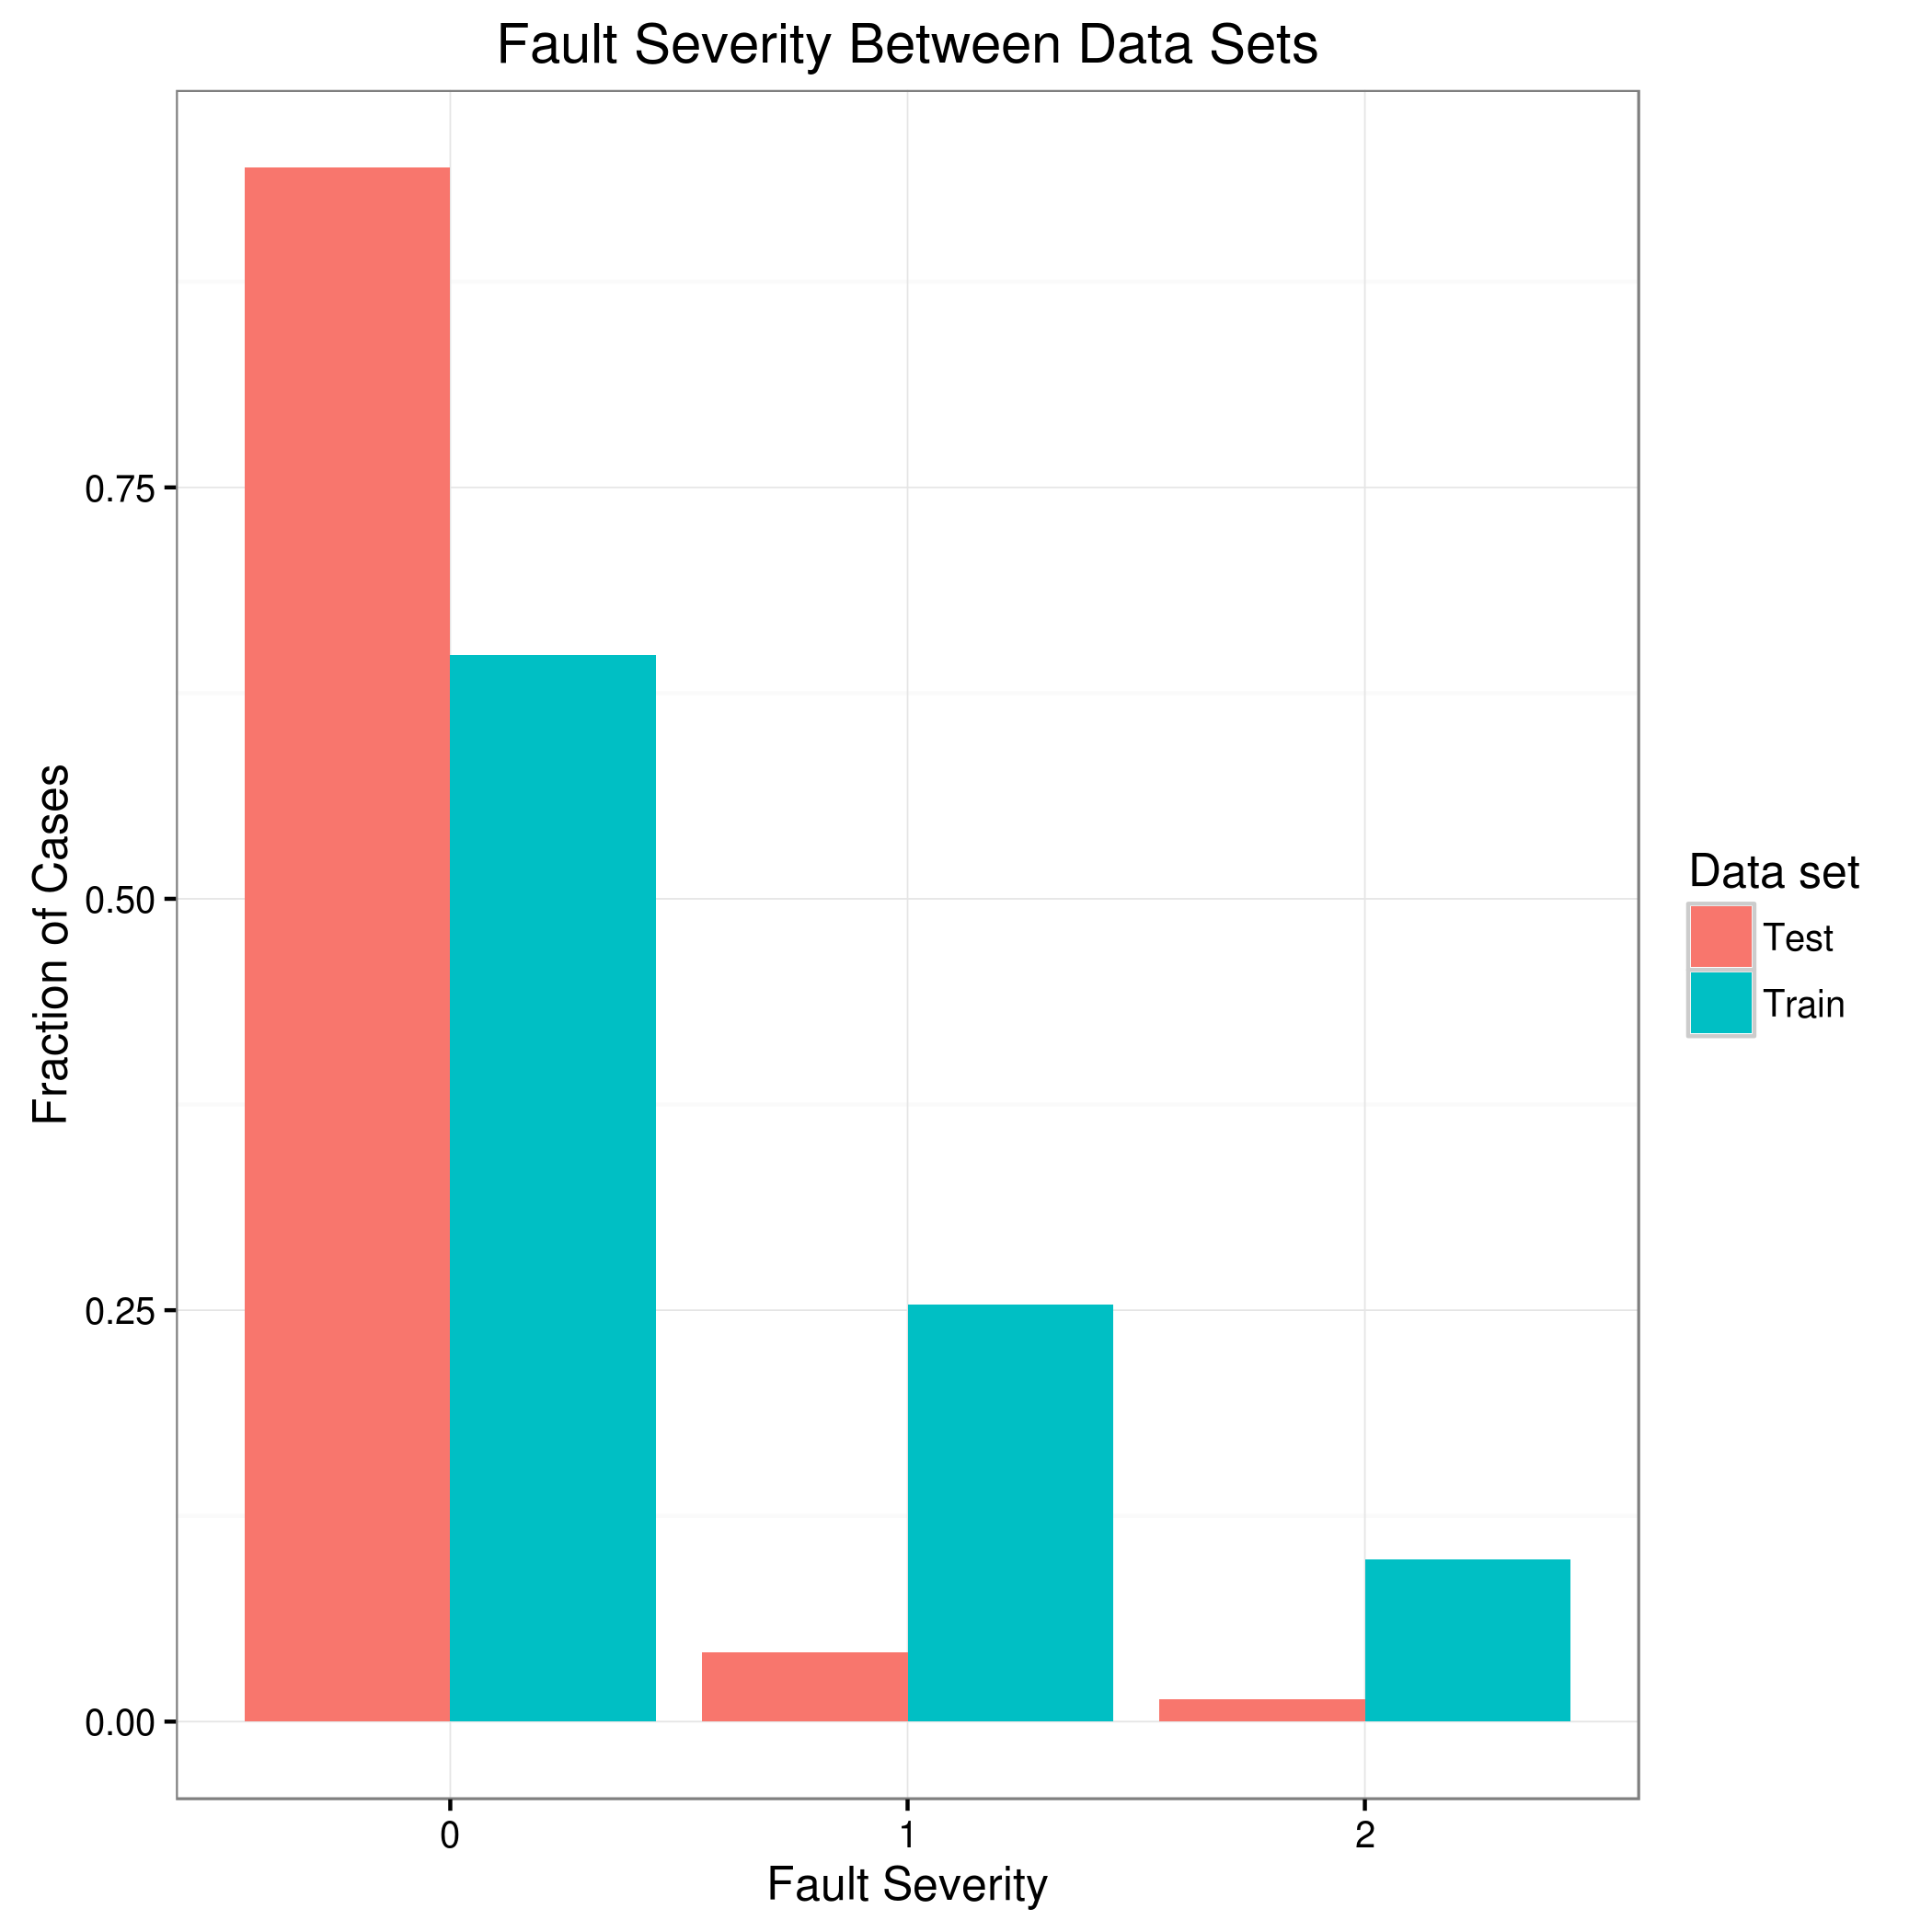
\includegraphics[scale=0.6]{Data/p_comp_frac.png}\end{centering}\\\\
These results had an internally computed (out of the bag error) accuracy of 69.64\%, and a kappa value, which is used to evaluate classifiers by comparing expected and observed accuracy, of 0.3436. Although the kappa value, is fairly low, an accuracy value of 69.64\% is impressive for such a sparse starting matrix.

\section*{Discussion and Conclusion}
Bagging was used to obtain reasonable predictions, as using random forests without bagging yielded uniform predictions of fault severity 0. We suspect this was due to the sparse nature of the starting data. However, we were also forced to use every feature to get some non zero predictions. Unfortunately, this negatively impacted predictive power.

To validate our results, we attempted to use another implementation of random forests without bagging (using the randomForest package in R) and predicted a single case with fault severity of 0, two cases with fault severity 1, zero cases of fault severity 2, and 11168 cases of NA fault severity. This indicates the naive approach using random forests is unsuited for this task.

Even though the Kaggle challenge had ended, we were not provided a gold standard file to compare our results with, so we lacked a measure of correctness for our analysis. If we were participating in the actual Kaggle challenge, our submitted results would be compared with such a file and we would receive a score (multiclass log loss) indicating any deviation from the gold standard. We were unable to compute such a value, so we cannot gauge the exact correctness of our results, or how our analysis compared to others in the competition.

Although we were unable to robustly check our results against a set of correct answers, we were able to predict fault severity with 69.64\% accuracy with a kappa value of 0.3436. Although not perfect, we’ve shown our approach is a suitable starting place for more in depth analyses.

\section*{Appendix}
\begin{enumerate}
\item Telstra Kaggle Challenge: \url{https://www.kaggle.com/c/telstra-recruiting-network}
\item Project Github Repository: \url{https://github.com/albertxu1994/math189_winter2016/tree/master/final}
\end{enumerate}

\end{document}
